% Limpa cabeçalhos.
% (solução para lidar com a númeração das páginas pré-textuais).
\pagestyle{empty}

% ----------------------------------------------------------
% ELEMENTOS PRÉ-TEXTUAIS
% ----------------------------------------------------------

%============================ Início da capa ============================================
\begin{center}
%--------------------------------------------
\begin{figure}[h!]
\parbox{2.5cm}{
\includegraphics[scale=0.15]{ufpi.jpg}}%
\quad
\begin{minipage}{12cm}%
\vspace{1cm}
\textsc{\large UNIVERSIDADE FEDERAL DO PIAUÍ}\\
\textsc{\large CENTRO DE TECNOLOGIA}\\
\textsc{\large BACHARELADO EM ENGENHARIA ELÉTRICA}\\
\end{minipage} %
\end{figure}
\vspace{4cm}
%nome do aluno
\textbf{\large WILK COELHO MAIA}\\
\vspace{4cm}
%título tcc
\textbf{\large PROJETO DE UM \textit{FRONT-END} ANALÓGICO PARA ETIQUETAS PASSIVAS \textit{RFID}}\\
\vfill
\textsc{\large teresina - piauí, \today}\\
\end{center}
\clearpage
%=========================== Fim da capa ===================================================


%============================ Início da página de rosto ============================================
\begin{center}
%----------------------------------------------------
\textbf{\Large WILK COELHO MAIA}
\par
\vspace{4cm}
\textbf{\Large PROJETO DE UM \textit{FRONT-END} ANALÓGICO PARA ETIQUETAS PASSIVAS \textit{RFID}}
\end{center}
\par
\vspace{4cm}
\hspace*{160pt}\parbox{9cm}{{Trabalho de conclusão de curso apresentado como requisito parcial para a obtenção do título de Bacharel em Engenharia Elétrica, pelo curso de Engenharia Elétrica da Universidade Federal do Piauí - UFPI.}}
\vspace{2cm}
\par\hspace*{160pt}\parbox{10cm}{Orientador: Prof. Dr. Marcos Eduardo do Prado Villarroel Zurita}
%\vspace{-0.3cm}
%\par\hspace*{160pt}\parbox{10cm}{Co-orientador: Nome do Co-orientador}
\vfill
\begin{center}
\textsc{\large teresina - piauí, \today}\\
\end{center}
\newpage
%============================ Fim da página de rosto ============================================


%============================ Início da folha de aprovação ============================================
\begin{center}
%----------------------------------------------------
\textbf{\Large WILK COELHO MAIA}
\par
\vspace{2cm}
\textbf{\Large PROJETO DE UM \textit{FRONT-END} ANALÓGICO PARA ETIQUETAS PASSIVAS \textit{RFID}}
\end{center}
\par
\vspace{1cm}
\hspace*{160pt}\parbox{9cm}{{Trabalho de conclusão de curso apresentado como requisito parcial para a obtenção do título de Bacharel em Engenharia Elétrica, pelo curso de Engenharia Elétrica da Universidade Federal do Piauí - UFPI.}}
\vspace{1.75cm}
\par\hspace*{160pt}\parbox{10cm}{Orientador: Prof. Dr. Marcos Eduardo do Prado Villarroel Zurita}
%\vspace{-0.3cm}
%\par\hspace*{160pt}\parbox{10cm}{Co-orientador: Nome do Co-orientador}
\vspace{1cm}
\begin{center}
Aprovado em 23 de janeiro de 2017.
\vspace{1.5cm}

BANCA EXAMINADORA
\vspace{0.5cm}

\begin{figure*}[!htb]
	\begin{center}
		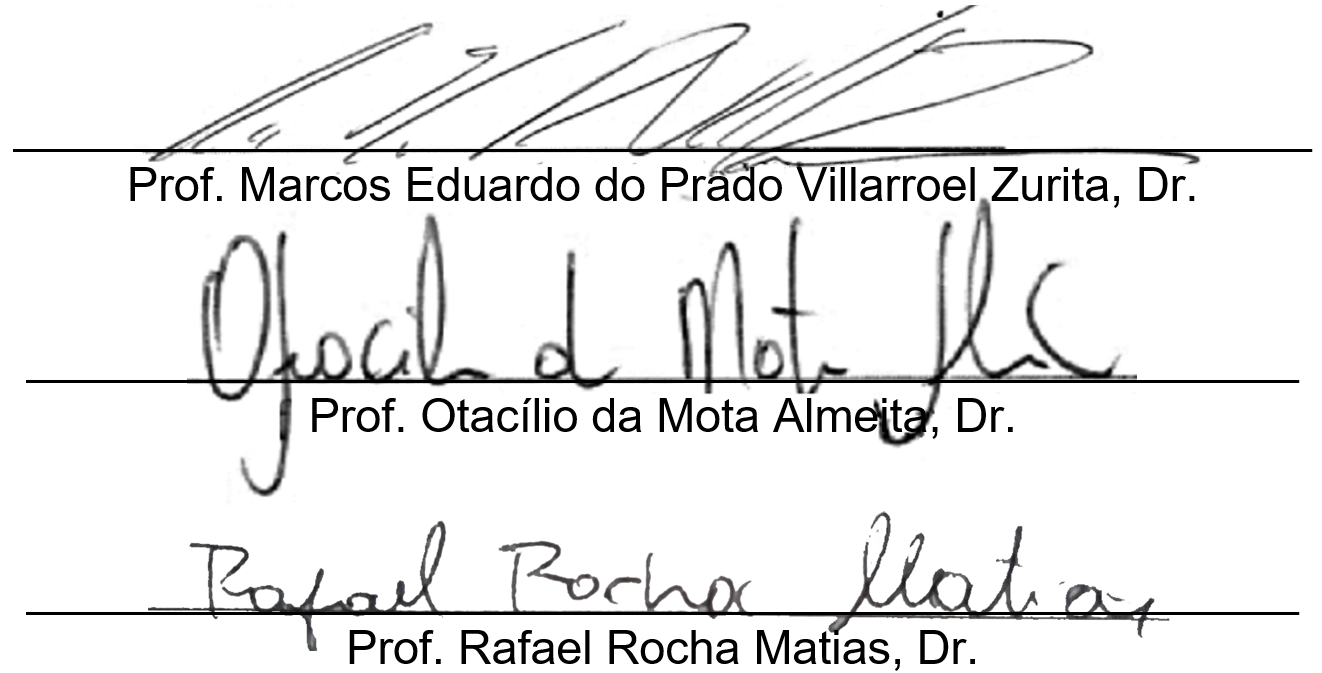
\includegraphics[width=.8\linewidth]{assinaturas.png}
	\end{center}
\end{figure*}

%\rule{14cm}{1pt}\\
%Prof. Marcos Eduardo do Prado Villarroel Zurita, Dr.
%\vspace{1cm}

%\rule{14cm}{1pt}\\
%Prof. Otacílio da Mota Almeida, Dr.
%\vspace{1cm}

%\rule{14cm}{1pt}\\
%Prof. Rafael Rocha Matias, Dr.

\end{center}
\clearpage
%============================ Fim da folha de aprovação ============================================

%-------------- AGRADECIMENTO + RESUMO + ABSTRACT ----------------------------------

\noindent{\LARGE\textbf{Agradecimentos}}

A Deus pelos caminhos que até aqui me trouxeram.

À minha família pelo apoio incondicional, pelo suporte sempre prestado e pelo amor a mim dedicado.

Aos professores do curso que me ajudaram e guiaram nos momentos de incerteza, em especial ao professor orientador pela ajuda nesta caminhada.

Aos colegas e amigos Francisco Victor e Andrei Carvalho. Sem vocês esta página estaria em branco.

\newpage

\vspace*{10pt}
% Resumo
\begin{center}
  \emph{\begin{large}Resumo\end{large}}\label{resumo}
\vspace{2pt}
\end{center}
% Pode parecer estranho, mas colocar uma frase por linha ajuda a organizar e reescrever o texto quando necessário.
% Além disso, ajuda se você estiver comparando versões diferentes do mesmo texto.
% Para separar parágrafos utilize uma linha em branco.
\noindent
Por décadas, aplicações nos campos militar e civil demandam melhoria no desempenho de dispositivos eletrônicos.
A constante evolução da sua tecnologia de desenvolvimento vem possibilitando o aumento significativo do desempenho alcançado por eles e, simultaneamente, a redução da energia demandada em seu funcionamento.
A utilização de etiquetas passivas RFID já é uma realidade em diversos setores, com aplicações que variam do comércio ao setor de segurança.
Este trabalho apresenta o projeto e resultados de simulação de um \textit{front-end} analógico para etiquetas desse tipo.
São projetados e implementados, em nível de simulação, os módulos responsáveis pela obtenção de energia a partir de um sinal de radiofrequência captado pela etiqueta e por alimentar seus demais módulos.
Foi utilizada tecnologia CMOS IBM 8RF 130 nm para o projeto e simulação de um retificador, referenciais de tensão e corrente e retificadores.
Os módulos são analisados e simulados individualmente e, posteriormente, em conjunto.
O resultado final obtido foi um dispositivo genérico que pode ser utilizado em etiquetas para diversas aplicações.
\par
\vspace{1em}
\noindent\textbf{Palavras-chave:} RFID, Front-end, Etiqueta passiva.
\newpage

% Criei a página do abstract na mão, por isso tem bem mais comandos do que o resumo acima, apesar de serem idênticas.
\vspace*{10pt}
% Abstract
\begin{center}
  \emph{\begin{large}Abstract\end{large}}\label{abstract}
\vspace{2pt}
\end{center}

% Selecionar a linguagem acerta os padrões de hifenação diferentes entre inglês e português.
\selectlanguage{english}
\noindent
For decades, applications on military and civil fields demanded performance enhancements of electronic devices.
The continual evolution on its development technology enables the significant growth on performance achieved by them and, simultaneously, a cutback on demanded energy.
RFID passive tags are already a fact on many areas, with applications ranging from commerce to security.
This work presents the project and simmulation results of an analog front-end for such tags.
The modules responsible for energy harvesting from incoming waves and for supplying power to specific modules of each tag are projected and implemented, on simulation level.
CMOS IBM 8RF 130 nm techonology was used for the project and simulation of a rectifier, voltage and current references and rectifiers.
The modules are analyzed and simulated individually and, afterawrds, together.
The result obtained was a generic device that can be used in many kinds of tags.
\par
\vspace{1em}
\noindent\textbf{Keywords:} RFID, Front-end, Passive tag.
\selectlanguage{brazil}
\clearpage
%-----------------------------------------------------------------------------------

\clearpage
\pdfbookmark{List of Figures}{lof} % Sets a PDF bookmark for the List of Figures
\listoffigures*

\clearpage
\pdfbookmark{List of Tables}{lot} % Sets a PDF bookmark for the List of Tables
\listoftables*

\clearpage
\renewcommand{\listadesiglasname}{Lista de siglas e abreviaturas}
\begin{siglas}
	\item[RFID] \textit{Radio-Frequency Identification}
	\item[EPC] \textit{Electronic Product Code}
	\item[TTL] \textit{Transistor-Transistor Logic}
	\item[ECL] \textit{Emitter-Coupled Logic}
	\item[CMOS] \textit{Complementary MOS}
	\item[BiCMOS] \textit{Bipolar-Complementary MOS}
	\item[MOS] \textit{Metal Oxide Semiconductor}
	\item[NMOS] Transistor MOS de canal N
	\item[PMOS] Transistor MOS de canal P
	\item[CC] Corrente Contínua
	\item[CA] Corrente Alternada
	\item[PTAT] \textit{Proportional To Absolute Temperature}
	\item[CTAT] \textit{Complementary To Absolute Temperature}
\end{siglas}

\clearpage
\pdfbookmark{\contentsname}{contents} % Sets a PDF bookmark for the Table of Contents
\tableofcontents*

\clearpage